\subsection{Kinosternidae --- Musk and Mud Turtles}
\begin{center}
\begin{longtabu} to \textwidth {| | p{3.5cm} | X | |}
	\hline
	Taxonomy/Ancestry &
	\begin{itemize}[noitemsep]
		\item 24 species within 4 genera, but taxonomic reclassification ongoing
		\item \emph{kinosternon} --- ``mud turtles," small aquatic turtles from the Americas
		\item \emph{sternotherus} --- ``musk turtles," endemic to N. America, closely related to \emph{kinosternon}
		\item \emph{claudius} --- only extant species is narrow-bridged musk turtle found in Mexico, Guatemala, and Belize
		\item \emph{staurotypus} --- Mexican musk turtles; giant musk turtles; three-kelled musk turtles; 2 recognized species found in Mexico and Central America
	\end{itemize}
	
	\begin{center} 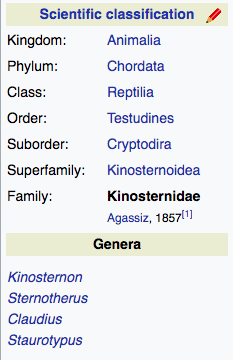
\includegraphics[scale=0.5]{testudines/kinosternidae/tax} \end{center}
	 \\
	\hline
	Size & 
	typically small, 10-15 cm (3.9-5.9 in) in length, but \emph{staurotypus} can get much larger, up to 30 cm (12 in).
	\\
	\hline
	Color &
	may be black, green, or yellowish in color. 
	
	most species don?t have shell markings, but some have radiating black markings on each carapace scute. some species have distinctive yellow striping along head and neck.
	 \\
	\hline
	Anatomy &
	\begin{itemize}[noitemsep]
		\item tall, highly domed upper carapace w/ distinct keel down center
		\item plastron differs by species
			\begin{itemize}[noitemsep] 
				\item some species have 1 or 2 hinges reaching from left to right side of shell; other species have none. the hinges allow plastron and carapace to pull tight against each other after the turtle pulls itself into the shell.
				\item some species have plastron covering only part of lower body; others have large plastron almost entirely concealing undersides
			\end{itemize}
		\item barbles* hanging from chin
		\item glands/sacs along side produce characteristic musky substance (smells like skunk spray)
	\end{itemize}
	 \\
	\hline
	Dimorphism & 
	Males usually have thicker and longer tails tipped w/ a spine; also have 2 rough, scaly patches on each leg. females are typically larger than males.
	\\
	\hline
	Behavior & 
	\begin{itemize}[noitemsep]
		\item aquatic for majority of lifespan
		\item slow swimmers
		\item travel to land for nesting or to feed during rainy season
		\item some diurnal, others nocturnal
		\item hibernation/estivation:
			\begin{itemize}[noitemsep]
				\item yellow mud turtle holds record for amt of time spent hibernating/estivating: inactive from winter to spring, summer to fall, only awakening when spring rains flood ground
				\item warm, wet climates --> active all year
				\item cold winters and deserts w/ long stretches of dry weather --> active only a few months a year and spend the rest underground waiting for better conditions
			\end{itemize}
		\end{itemize}
				
	\\
	\hline
	Habitat & 
	freshwater species living in still or slow-moving waters. prefer year-round bodies such as lakes or ponds. a few reside in shallow, seasonal ponds which have water only during a few months of the year, typically spring.
	\\
	\hline
	Distribution & 
	native to Americas
	\\
	\hline
	Feeding Ecology & 
	carnivorous turtles eating snails, clams, insects, worms, leeches, and sometimes freshly killed fishes they find. those w/ large heads typically prefer snails and clams which they can easily open w/ their jaws. in seasonal ponds, they may eat a large amount of seeds.
	\\
	\hline
	Reproductive Biology & 
	\begin{itemize}[noitemsep]
		\item no courtship rituals; mating takes place in water
		\item females go onto land to nest. they may either bury eggs in a hole they dig or simply lay eggs on surface leaves.
		\item lay 3-6 hard-shelled eggs during late spring and early summer
		\item up to 6 clutches per year
		\item oblong eggs range from 0.9-1.7 in (2.3-4.3 cm) long and from 0.6-1.0 in (1.5-2.5 cm) wide
		\item hatch 75 days to a year after being laid
		\item TSD: medium temperatures produce male offspring; females are produced by extremes
		\item post-eclosion, some species winter in subterranean nest and truly emerge in spring
		\item the yellow musk turtle is the only turtle species known to exhibit parental care. suggested to sometimes stay w/ nest and urinate on eggs long after laying to keep them moist or protect them from predators.
	\end{itemize}
	\\
	\hline
	Ecological Role &
	
	\\
	\hline
	Conservation Status & 
	4 VU; US Fish and Wildlife lists flatted musk turtle as Threatened. However, most species are quite common in their own habitats.
	\\
	\hline
\end{longtabu}
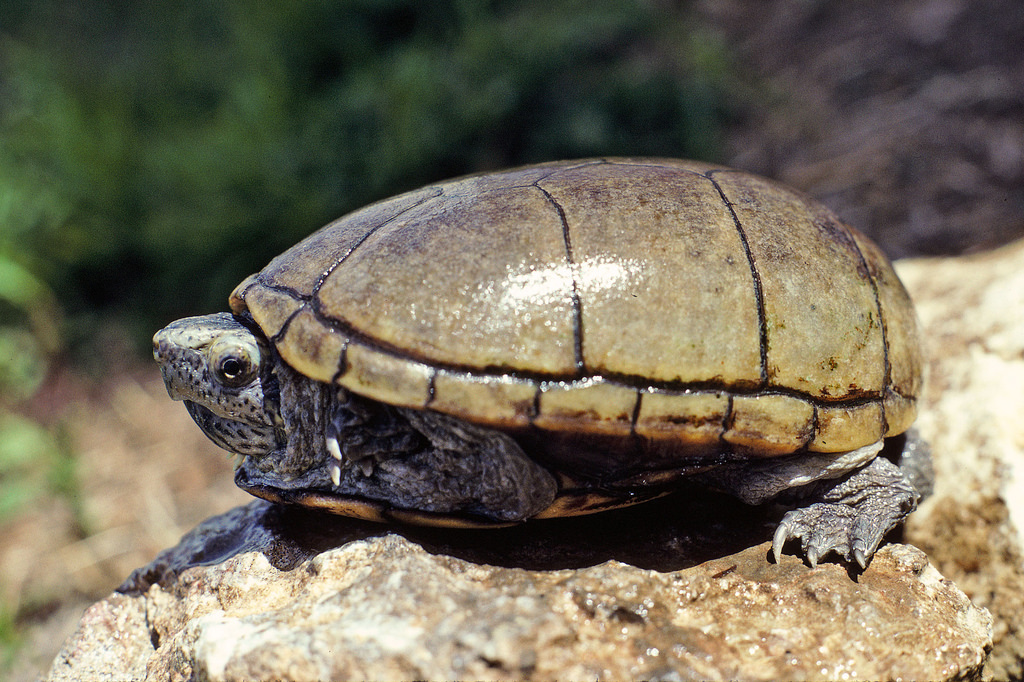
\includegraphics[scale=0.25]{testudines/kinosternidae/kino1}
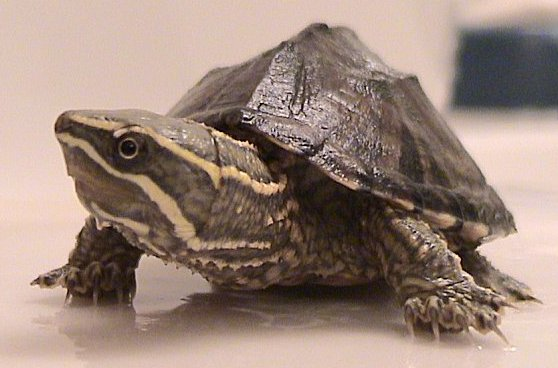
\includegraphics[scale=0.5]{testudines/kinosternidae/kino2}
\end{center}
